\chapter{Detector and Focal Plane Design}\label{c:det-design}

This chapter describes the design of the \Imager's detectors and focal plane.
Prior to fabrication of the 251-detector sub-array that is discussed in this dissertation, prototype detectors were fabricated and characterized.
Because the measured properties of the prototype detectors are relevant to some of the parameter choices made for the sub-array detectors, this chapter begins with a short summary of the measured properties of those detectors.
I then discuss the choice of parameters $G$, $C$, $T_c$ and $T_b$ for the sub-array detectors, the choice of shunt resistor value $R_{sh}$ and Nyquist inductor $L$, followed by details of the detector design used to achieve these parameters.
I then briefly describe the design of the focal plane, and end with the predicted detector noise and \NETD\ for the system.

\section{Prototype Detectors} \label{sec:det-parm-choice}

The basic design and layout of the prototype detectors was the same as described in \sectionref{sec:ch5-det-design} for the sub-array detectors.
Four prototype detectors were tested both in the dark and while open optically, and also used to take still images.
The techniques used to characterize the prototype detectors were the same as those use to characterize the sub-array detectors, as described in \chapterref{c:det-array}.
\tableref{tab:ch5-proto-parms} lists parameters of these detectors, and \figref{fig:ch5-proto-plots} contains plots showing \Loop, $\beta_I$, $\tau_{eff}$ and $L_{crit}$ for these detectors, measured at a range of bias points.

\begin{table*}
\centering
\caption[Measured properties of prototype detectors]{
  Measured Properties of Prototype Detectors.
  The methods and procedures used to measure these properties were the same as described for the sub-array in \chapterref{c:det-array}.
} 
\label{tab:ch5-proto-parms}
\begin{tabular}{l c}
\toprule
  Detector Property &  {Value} \\
\midrule
  $T_c$                 & \SI{1.2}{\K} \\
  $R_n$                 & \SI{3.4}{\mOhm} \\
  $n$                   & 3.9 \\
  $G$                   & \SI{5}{\nW\per\K} \\
  $\tau$                & \SI{12}{\ms} \\
  $\tau_{eff}$ (typical) & \SI{4}{\ms} \\
  $C = G \tau $         & \SI{60}{\pJ\per\K} \\
  $P_{opt}$              & \SI{150}{\pW\per\K} \\
  $\eta_{tot}$           & 0.25 \\
  $P_{sat}|_{\SI{970}{\mK}}$          & \SI{920}{\pW} \\
\bottomrule
\end{tabular}
\end{table*}

\begin{figure*}
\centering
\includegraphics{drawings/ch5-proto-plots.pdf}
\caption[Plots of \Loop, $\beta_I$, $\tau_{eff}$ and $L_{crit}$ for prototype detectors]{
  Plots showing \Loop, $\beta_I$, $\tau_{eff}$ and $L_{crit}$ vs bias point for four prototype detectors.
  \Loop,  $\beta_I$, and $\tau_{eff}$ were measured using the same techniques described in \chapterref{c:det-array}.
  The values of $L_{crit}$ were calculated using \eqnref{eqn:ch3-L-stable}.
}
\label{fig:ch5-proto-plots}
\end{figure*}

\section{Bolometer Design Parameters} \label{sec:det-parm-choice}

The primary parameters to be chosen when designing a \TES\ bolometer are the superconducting critical temperature $T_c$, the thermal conductance $G$, and the \TES\ island heat capacity $C$.
These parameters are interrelated, and so cannot be chosen independently of each other.
Some of the factors to consider are:
\begin{itemize}
  \item Detector noise scales with $\sqrt{T_c^2 G}$, so that lower values of $G$ and $T_c$ improve noise.
  \item As discussed in \sectionref{sec:ch3-psat}, the saturation power of the \TES\ detector scales roughly like $G T_c$, so that if $G$ and $T_c$ are too small, the optical power falling on the detector will raise the temperature of the membrane above $T_c$, saturating the device and rendering it inoperable.
  \item $T_c$ must be chosen to be higher than the achievable bath temperature, and the bath temperature also affects the saturation power through \eqnref{eqn:ch3-p-bath}.
  \item The detector time constant $\tau_{eff}$ is proportional to the detector natural time constant $\tau = C / G$.
\end{itemize}

% xxx say something about no attempt to shape transition - we get whatever alpha we get. no need to slow down trans, which is what normal metal bars do.

The following subsections outline the choice of $T_b$, $T_c$, $G$ and $C$ for the detectors in the first 251-detector sub-array.

\subsection{Choice of $T_b$ and $T_c$}

The relationship between detector noise and saturation power can be examined in more detail.
From \eqnref{eqn:ch3-psat} we have
\begin{equation} \label{eqn:ch5-psat}
P_{sat} = \frac{G T_c}{n}\left(1 - \left(\frac{T_b}{T_c}\right)^n\right).
\end{equation}
This can be solved for $G$ and substituted into the expression for \TES\ thermal fluctuation noise in \tableref{tab:tes-noise}, leading to
\begin{equation} \label{eqn:ch5-tes-noise}
S^2_{TFN} = \frac{n F(T_c, T_b) }{\frac{T_b}{T_c} \left( 1-(T_b/T_c)^n \right)} 4 \, k_B T_b P_{sat}.
\end{equation}
The \TES\ temperature $T_c$ appears only in the pre-factor, which depends only on the power-flow index $n$, the ratio $T_b/T_c$, and the form of $F$.
This means that for fixed $P_{sat}$ and $T_b$, the ratio $T_c/T_b$ that gives the lowest detector noise depends only on $n$ and the form of $F$.
For values of $n$ in the range 3--4, this optimal ratio is $T_c \approx 1.8 T_b$, while the pre-factor itself is \abt{3.7}.

As discussed in \sectionref{sec:ch4-opt-eff}, the predicted loading on the \Imager's detectors is \SI{180}{\pW} and the photon noise from this load is \Pnoisef{0.85}.
Choosing a safety factor of 3 so that $P_{sat} = 3 \times \SI{180}{\pW}$, and targeting detector noise equal to \SI{50}{\percent} of the photon noise (so that total noise is a factor of $\sqrt{1.5} = 1.22$ higher than photon noise), we find the requirement on $T_b$ to be
\begin{equation}
  T_b < \frac{1}{3.7} \frac{\NEPph^2}{4 k_B P_{sat}} =
        \frac{1}{3.7} \frac{0.5 \times (\num{0.85e-15})^2}{4 \times \SI{1.38e-23}{\J\per\K} \times 3 \times \SI{180}{\pW}} = 
        \SI{3.6}{\K}
\end{equation}

A \SI{3.6}{\K} bath temperature can be reached through the use of solely a mechanical cryocooler, which would simplify the design of the cryostat.
However, this leaves little margin for error in the design and implementation of the system, so for the \Imager\ we chose to use a \He4-sorption fridge to allow setting the bath temperature well below \SI{3.6}{\K}.

The initial hopes for performance of the \He4-sorption fridge were that its base temperature would be \abt{\SI{650}{\mK}}, implying an ideal $T_c$ of \abt{\SI{1.2}{\K}}.
This is a convenient $T_c$ because it is the critical temperature of elemental Al \cite{matthias_superconductivity_1963}, so Al was chosen as the \TES\ material.

In practice, it was discovered during testing of the prototype detectors that the base temperature of the system was \SI{950}{\mK} under optical load, not \SI{650}{\mK}.
With a bath temperature of \SI{950}{\mK}, the optimal choice of $T_c$ would be \abt{\SI{1.7}{\K}}; this higher $T_c$ would allow a lower $G$ to be used so that thermal fluctuation noise of the detectors would decrease.
However, in order to change as little as possible between the prototype detectors and the first sub-array, I decided to continue using Al as the \TES\ material.

\subsection{Choice of $G$}

\tableref{tab:ch5-proto-parms} lists the measured properties and parameters of the prototype detectors.
These detectors had $P_{sat}$ at $T_b = \SI{970}{\mK}$, 5.1 times higher than the predicted optical load and 6.1 times the measured optical load.
A safety factor of 5--6 is overly conservative, so for the sub-array I decided to target a $G$ value of \SI{3.8}{\nW\per\K}, for a safety factor of 3.9 -- 4.7.

\subsection{Choice of $C$}

The detector's heat capacity $C$ is chosen to target a specific detector time constant $\tau_{eff}$ once $G$ is chosen.
$G$ and $C$ do not set $\tau_{eff}$ directly, rather they set the natural time constant $\tau$, to which $\tau_{eff}$ is proportional via \eqnref{eqn:teff}.
$\tau_{eff}$ must be fast enough to avoid blurring of video-rate images, but should be much larger than $\tau_{el}$ to avoid detector instability; see \sectionref{sec:ch3-tes-stability}.

We can estimate the required value of $\tau_{eff}$ by considering the speed with which detectors move on the far-field focal plane and the size of the far-field beam.
If $v$ is the speed with which the detector far-field beam moves, and $b_{fwhm}$ is the \FWHM\ far-field beam width, then scanning over a point source will result in a timestream with a Gaussian ``bump'' with \FWHM\ $q_{raw} \equiv b_{fwhm} / v$.
The \TES\ acts like a lowpass filter on this timestream with time constant $\tau_{eff}$.
The timestream after filtering is given by the convolution%
\footnote{The factor 2.35 converts the \FWHM\ of the timestream bump to the ``standard deviation'' term for the Gaussian.}
\begin{equation}
  d_{filt}(t) = \int_{-\infty}^{t} \exp{\left[-\frac{2.35^2}{2} \frac{{t^{\prime}}^2}{(b_{fwhm}/v)^2}\right]}
       \exp{\left[-(t-t^{\prime})/\tau_{eff}\right]} dt^{\prime}.
\end{equation}
The \FWHM\ of the bump after filtering will be $q_{filt}$.
We can quantify the amount of blurring with a fractional blurring factor $(q_{filt} - q_{raw})/q_{raw}$.

As shown in \sectionref{sec:ch5-fov}, when scanned circularly the detectors trace out a circle of radius \SI{18.7}{\cm}.
If $FPS$ is the video frame rate, then $v$ will be given by $(2 \pi)(\SI{18.7}{\cm}) FPS$.
From \sectionref{sec:ch4-feedhorn-design}, the predicted beam \FWHM\ is \SI{1.4}{\cm}.
\figref{fig:ch5-teff-bump} shows what value of $\tau_{eff}$ is required in order to achieve a given blurring factor, for three different frame rates (6, 10, and 20 frames per second).

\begin{figure*}
\centering
\includegraphics{drawings/ch5-teff-bump.pdf}
\caption[Maximum $\tau_{eff}$ for no blurring]{
  Plot of maximum allowed $\tau_{eff}$ as a function of fractional blurring factor, defined in the text, for three different video frame rates.
}
\label{fig:ch5-teff-bump}
\end{figure*}

If we take \SI{10}{\percent} as the maximum desired fractional blurring factor, then $\tau_{eff}$ must be \SI{0.14}{\ms} or faster to avoid blurring at 20 frames per second.
From \tableref{tab:ch5-proto-parms} this is \abt{30} times faster than the measured values for the prototype detectors.
At 6 frames per second the requirement on $\tau_{eff}$ is \SI{0.5}{\ms}, \abt{8} times faster than the prototype detectors.

Either of these target values for $\tau_{eff}$ could be reached by reducing the thickness of the Au ring.
However, such a large decrease in the detector time constant risks detector instability, and I did not want to risk losing an entire wafer of detectors due to instability.
For that reason I decided to reduce $C$ by a factor of only 2, by cutting the thickness of the Au ring in half.
Given the design $G = \SI{3.8}{\nW\per\K}$, and the prototype value of $C = \SI{60}{\pW\per\K}$, this should give $\tau = \SI{7.9}{\ms}$, assuming the same properties for Au in the prototype detectors and the sub-arrays. 
As long as \Loop\ and $\beta_I$ at the operating bias point did not change from the prototype detectors, this would reduce $\tau_{eff}$ to $\SI{4}{\ms} \times \frac{7.9}{12} = \SI{2.6}{\ms}$.
$C$ for subsequent sub-array fabrications can be adjusted lower based on the measurements of the first fabricated sub-array.

\section{Detector Geometry} \label{sec:ch5-det-design}

The \Imager's detectors are fabricated using standard lithographic clean-room techniques on Si wafers.
In order to achieve the targeted $G$ and $C$ values, the detectors are located on a suspended SiN membrane which is connected to the rest of the Si wafer by a set of thin SiN ``legs''.
\figref{fig:ch5-det-layout} shows a cross-sectional schematic of the detectors, showing that they are suspended with no Si beneath them, as well as a labeled photograph of a prototype detector.
The sub-array detectors are identical except for the length of the legs and the thickness of some of the layers; see \tableref{tab:ch5-det-dims}.

\begin{figure*}
\centering
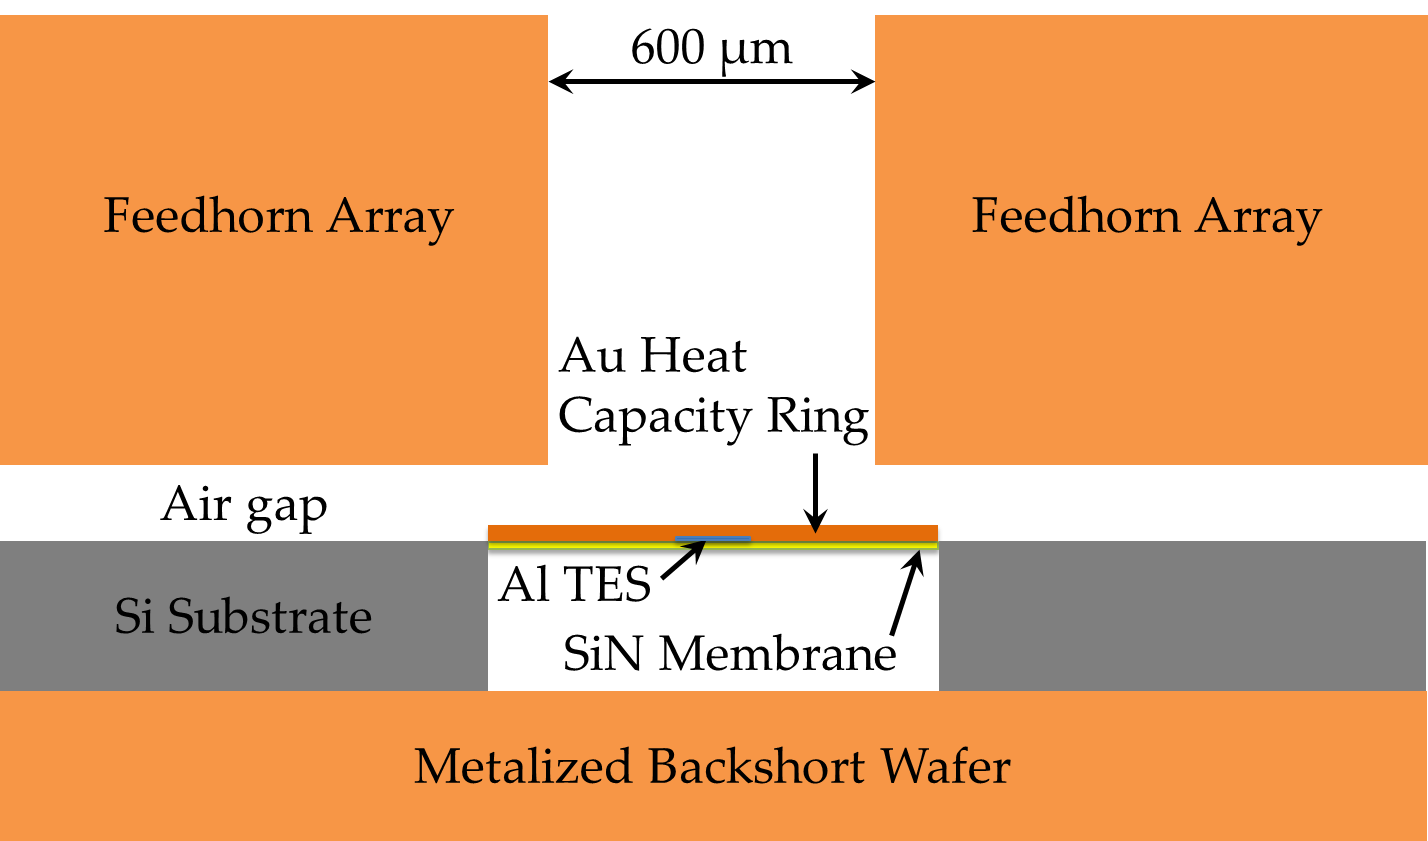
\includegraphics[width=3.9in]{images/ch5-det-schematic.png}
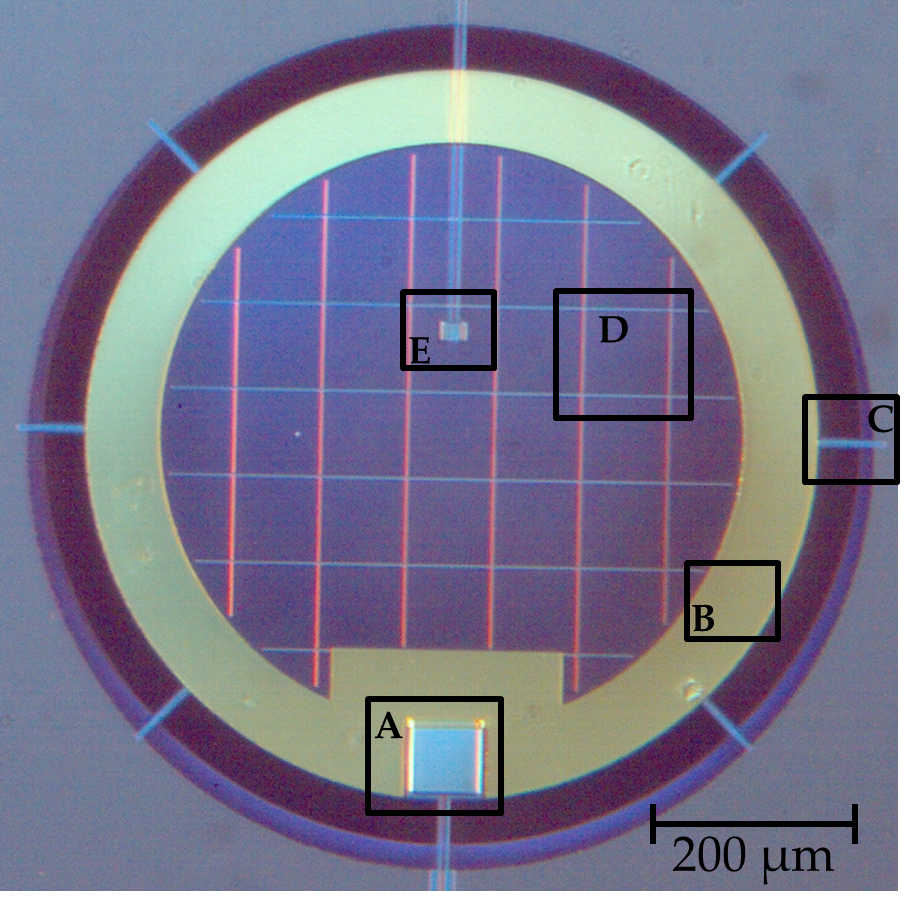
\includegraphics[width=2.3in]{images/ch5-proto-pixel-labeled.png}
\caption[Detector cross-section and photograph]{
  \textbf{Left} Cross-sectional schematic of a \Imager\ detector.
  Other than the thickness of the \TES, SiN membrane and Au Heat Capacity Ring, the schematic is to scale.
  \textbf{Right} Photograph of a prototype detector.
  The detectors fabricated for the sub-array are identical except for the length of the legs and the thickness of some of the layers; see \tableref{tab:ch5-det-dims}.
  The labeled parts of the detector are \textbf{A:} Al \TES\ \textbf{B:} Au heat capacity ring \textbf{C:} SiN leg connecting detector to substrate \textbf{D:} PdAu absorbing mesh \textbf{E:} PdAu heater resistor.
}
\label{fig:ch5-det-layout}
\end{figure*}

The detectors are fabricated on \SI{275}{\um} thick double-side-polished degenerate (Boron P-type) Si wafers.
A layer of SiO2 is grown on top of the Si, followed by a layer of SiN, prior to the main fabrication steps.
During fabrication the Nb wiring leads, Al \TES, PdAu absorber, and Au heat-capacity ring are deposited, as well as an additional layer of insulator to allow wiring layers to cross over each other.
The SiN and SiO2 is removed from the areas between the legs, and then a Deep Reactive Ion Etch process is used to remove all silicon from behind the detector membrane.
This etch process does not remove SiN or SiO2, so that the legs, which still have SiN, are left in place.
The result is a suspended membrane connected to the rest of the wafer by a set of ``legs'' which provide the thermal conductance $G$.

\tableref{tab:ch5-det-dims} lists dimensions for both the prototype and sub-array detectors.

% xxx important ... do the Nb leads contribute to G? No electrical
% contribution, but there should still be a lattice contrib, and that
% might be higher than the disordered SiN and SiO2 ...

The leg geometry of the prototype detectors was chosen based on a set of measurements taken at \NIST\ on SiN membranes at temperatures near \SI{1}{\K}.
The leg geometry for the sub-array detectors was based on simple scaling of the prototype detectors to the target $G$ of \SI{3.8}{\nW\per\K}.
This scaling was slightly complicated by the change in thickness of the SiO2 layers, which was made in order to add additional protection to the wiring layers and better balance stress on the relieved membranes.
Assuming that $G$ scales linearly with the $A/L$ of the legs, the sub-array $G$ should be
\begin{align}
  G_{sub} & = G_{proto} \frac{A_{sub}}{A_{proto}} \frac{l_{proto}}{l_{sub}} \\
         & = \SI{5.0}{\nW\per\K} \frac{(500 + 250 + 200)(11)}{(500 + 120 + 120)(11)} \frac{40}{67} \\
         & = \SI{3.8}{\nW\per\K} 
\end{align}

\begin{table*}
\centering
\caption[Detector dimensions]{
  Dimensions of prototype and sub-array detectors.
  For the sub-array, only values differing from the prototypes are shown.
} 
\label{tab:ch5-det-dims}
\begin{tabular}{l c c}
\toprule
  Detector Dimension &  {Prototype} & Sub-Array \\
\midrule
  \TES\ Size (l $\times$ w) & $\SI{64}{\um} \times \SI{70}{\um}$ & \\
  \TES\ Thickness      & \SI{250}{\nm}       & \SI{180}{\nm} \\
  SiN Thickness        & \SI{500}{\nm}       & \\
  SiO2 Base Thickness  & \SI{120}{\nm}       & \SI{250}{\nm} \\
  SiO2 Cover Thickness & \SI{120}{\nm}       & \SI{200}{\nm} \\
  Number of Legs       & 8                   & \\
  Leg Length           & \SI{40}{\um}        & \SI{67}{\um} \\
  Leg Width            & \SI{11}{\um}        & \\
  Au Ring Area       & $(\SI{393}{\um})^2$ & \\
  Au Ring Thickness  & \SI{2000}{\nm}      & \SI{1000}{\nm} \\
  Nb Lead Width        & \SI{6}{\um}         & \\
  Nb Lead Thickness    & \SI{200}{\nm}       & \\
  PdAu Thickness       & \SI{20}{\nm}        & \\
\bottomrule
\end{tabular}
\end{table*}

\tableref{tab:ch5-det-heat-capacity} shows contributions to the heat capacity from all components of the bolometer.
The membrane and Al \TES\ alone have insufficient heat capacity, so an Au ring was added to provide the targeted heat capacity.
The total heat capacity is dominated by the Au ring.

\begin{table*}
\centering
\caption[Detector heat capacity contributions]{
  Predicted contributions to total heat capacity of sub-array detectors.
  Note that the Debye $T^3$ contribution for Au is still significant at \SI{1.2}{\K}, so must not be ignored.
  All values listed are at \SI{1.2}{\K}.
} 
\label{tab:ch5-det-heat-capacity}
\begin{tabular}{l S S S l}
\toprule
  Component & {Volume ($10^{-9}$\,\si{\cm^3})} & {$C_V$ (\si{\uJ\per\K\per\cm^3})} & {$C_{tot}$ (\si{\uJ\per\K})} & Source \\
\midrule 
    SiN & 203.6 &   1.0 &   0.2 & \cite{holmes_measurements_1998} \\ 
   SiO2 & 183.2 &   3.1 &   0.6 & \cite{zeller_thermal_1971,zink_specific_2004} \\ 
     Al &   0.8 & 196.8 &   0.2 & \cite{irwin_transition-edge_2005} \\ 
     Au & 154.4 & 161.3 &  24.9 & \cite{corak_atomic_1955} \\ 
\midrule 
  Total &       &       &  25.8 \\ 
\bottomrule
\end{tabular}
\end{table*}

\section{Shunts and Nyquist Inductors} \label{sec:ch5-shunt}

The \Imager\ uses spare shunt resistors and Nyquist inductors originally made for the Atacama B-Mode Search (\ABS) project \cite{kusaka_modulation_2013}.
The design value for the shunt resistors was \SI{180}{\uOhm} and for the inductors \SI{609}{\nH}.
These chips were already fabricated and available, and the values of $R_{sh}$ and $L$ are appropriate for the \Imager's detectors.

The measured normal-state resistance of the prototype detectors was \SI{3.4}{\mOhm}, but the thickness of \TES\ material was reduced for the sub-array by \abt{\SI{30}{\percent}}, for a target sub-array normal-state resistance of \SI{3.9}{\mOhm}.
This allows $R_{sh}$ to be more than five times smaller than $R_0$ at bias points as low as $R_0 = 0.25 R_n$, allowing a robust voltage bias.

As shown in the lower right plot of \figref{fig:ch5-proto-plots}, the smallest value of $L_{crit}$ for any of the four prototype detectors across all bias points was \SI{2000}{\nH}.
This value drops to \SI{1300}{\nH} given the faster design value of $\tau$ for the sub-array detectors.
Therefore, $L = \SI{609}{\nH}$ is low enough to ensure that the sub-array detectors are stable, with a large safety margin in case the values of \Loop\, $\beta_I$, or $\tau$ changed between the prototype and sub-array.
Lower values of $L_{crit}$ would work as well, and may be considered if faster detector response times are targeted in a future iteration of this system.

\section{Detector Wafer Layout} \label{sec:ch5-layout}

\figref{fig:ch5-full-wafer} shows a photograph of the entire sub-array; the figure caption contains a detailed description of the features present on the sub-array.
In addition to the detectors, the wafer includes Au pads for attaching Au heat-sinking wire bonds and holes used for gluing the detector wafer to an Au-covered backshort wafer (see \sectionref{sec:ch5-focal-plane}).
Note that all detectors have heater resistors on their membranes, but only a subset have the resistors connected to traces that lead to bond pads due to space limitations on the wafer.

The detectors are laid out on a square grid, chosen over a hexagonal close-packed layout because of the simpler wiring layout.
The choice of a square grid does slightly compromise the system \NETD\ by \abt{\SI{5}{\percent}}, due to lower packing efficiency compared to a hexagonal array.
Higher packing efficiency allows larger feedhorns, which for the \Imager\ leads to higher spillover efficiency; see \figref{fig:ch4-feed-spill}.

%A hexagonal close-packed array would allow the same number of detectors to be placed on the array, but with feedhorns \SI{7.5}{\percent} larger.
%The larger feedhorn size could have improved the spillover efficiency from \num{0.52} to \num{0.544}, a \SI{4.6}{\percent} increase, leading to a \SI{4.6}{\percent} improvement in \NETD.

Five locations in the $16 \times 16$ grid are missing detectors.
The detector in the upper rightmost corner of \figref{fig:ch5-full-wafer} was removed to allow placement of a central post in the focal plane, to which the feedhorn array is bolted.
This provides an additional thermal link at the center of the feedhorn array for better heat sinking.
Four detectors in the lower left were removed to allow placement of alignment features on the detector wafer.
In practice these alignment features were not used, so some or all of these detectors could be recovered in a future design iteration.

\begin{figure*}
\centering
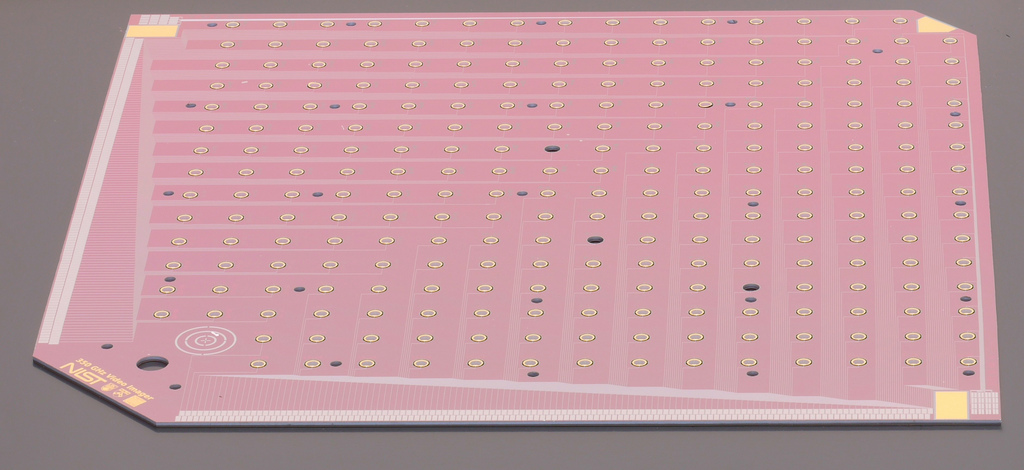
\includegraphics{drawings/ch5-full-wafer.pdf}
\caption[Photograph of 251-detector sub-array]{
  Photograph of the 251-detector sub-array.
  Bond pads for connecting to the detectors run along the left and bottom sides.
  In the upper left, lower right, and upper right corners are Au pads for connecting Au wire bonds to allow the wafer to be heat-sunk to the rest of the \SI{1}{\K} stage.
  The upper left and lower right corners also contain small bond pads for connecting to detector heaters.
  While all detectors have heater resistors on their membrane, only the detectors along the upper and right edges have these resistors wired to bond pads.
  The 26 small holes spaced throughout the wafer are used to glue the detector wafer to a backshort wafer (see text).
  The three larger holes in the middle of the wafer are detector sites where the membrane was broken during fabrication.
  The large hole in the lower left, as well as the ``bulls-eye'' feature to its immediate upper right, are alignment features, although they were not actually used.
  Photograph credit Dan Schmidt; full-resolution version available at \protect\url{http://www.flickr.com/photos/quantumsensors/8592792487}.
}
\label{fig:ch5-full-wafer}
\end{figure*}

\section{Focal Plane Design} \label{sec:ch5-focal-plane}

The \Imager's detector arrays are mounted on an Al platter that is thermally sunk to the cold head of the \He4-sorption fridge via a set of braided CU cables.
Mechanically the focal plane is attached to an Al frame via four Ti-6Al-4V ``spiders''.
The frame itself is bolted to the \SI{6}{\K} cold plate.
See \figref{fig:ch5-focal-plane-back}.

\begin{figure*}
\centering
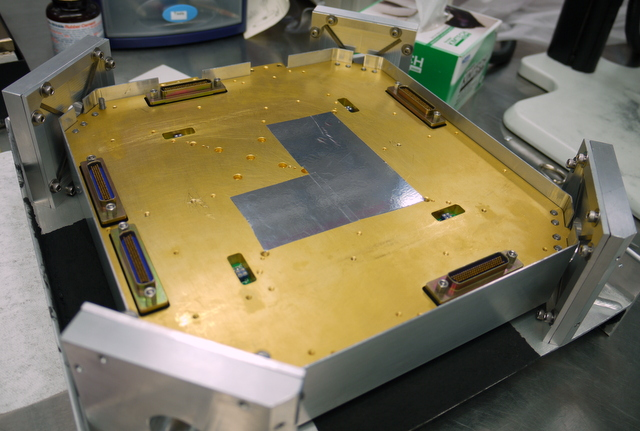
\includegraphics{drawings/ch5-focal-plane-back.pdf}
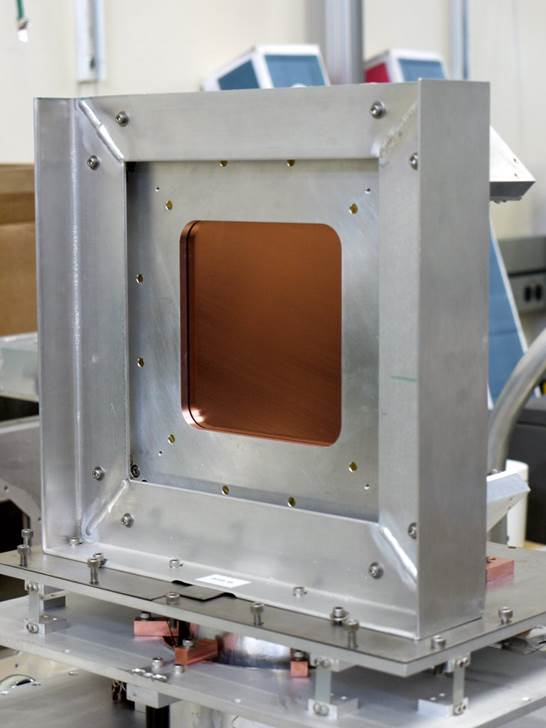
\includegraphics{drawings/ch5-focal-plane-cryostat.pdf}
\caption[Photograph of focal plane in cryostat]{
  Photographs showing how the focal plane is attached to the \SI{6}{\K} Cold Plate.
  \textbf{Left}
  Back view of the focal plane.
  \textbf{A:} Ti-6Al-4V ``spiders'' which provide the thermal and mechanical link between the focal plane and the \SI{6}{\K} Cold Plate.
  A spider is located at each corner of the focal plane, where it is clamped into an Al block.
  The Al blocks are then bolted to an Al frame.
  \textbf{B:} One of the 100-pin MDM connectors that the wires from the \MCE\ plug into.
  \textbf{C:} It is better for stray infrared light to be absorbed on the \SI{6}{\K} cold stage rather than the focal plane, so the Al frame has Berkeley Bock Black \cite{persky_review_1999} applied to it for \IR\ light absorption.
  \textbf{Right}
  Photograph of the Al frame and focal plane bolted onto the \SI{6}{\K} Cold Plate.
  The copper-colored area is the W1275 bandpass filter.
  \textbf{D:} Al frame.
  This photograph was taken prior to the application of the Berkeley Bock Black.
  \textbf{E:} The \SI{80}{\K} plate.
  Visible to the right of the \textbf{E} rectangle are the end-points of the Cu ropes that connect the \PTC\ 2nd-stage cold head to the \SI{80}{\K} plate.
}
\label{fig:ch5-focal-plane-back}
\end{figure*}

Each sub-array is glued to a \SI{275}{\um} thick Si ``backshort'' wafer that has been micro-machined to have the same outline as the sub-array and then covered with Au.
The glue used was Stycast 2850 with the LV 23 catalyst\footnote{Henkel Emerson \& Cuming, Billerica, MA}.
The glue was applied to the set of 26 holes in the detector wafer shown in \figref{fig:ch5-full-wafer}.
This wafer stack is then attached to an \SI{0.125}{\in} thick Invar plate.
Invar was chosen because its thermal contraction upon cooling is well-matched to Si \cite{ekin_experimental_2006}.
%Choosing a material that is poorly matched to Si could result in breaking the Si stack upon cooling.
The wafer stack is attached to the Invar plate with a thin layer of Apiezon-N thermal grease.
Upon cooling to cryogenic temperatures Apiezon N grease solidifies, so that the detector wafer will not slip along the Invar.
Even at room temperature the grease is very viscous, so that if the back of the wafer stack is entirely covered with a layer of grease the wafer will not slip under the influence of gravity if, e.g., it is stored facing horizontally in the cryostat while at room temperature.

The Invar plates must be attached to the Al platter in a way that accounts for the differential thermal contraction between Al and Invar, while ensuring that the detectors are correctly aligned to the feedhorns.
This is done by aligning the Invar, feedhorns, and Al platter to each other using stainless steel dowel pins.
Two pins align the feedhorns to the Al platter.
The dowel pins are inserted into the Al platter, with one matching hole and one matching slot in the feedhorn array; a slot is used for one of the holes to avoid over-constraining the mechanical system.
Two additional pins align each Invar plate to the Al platter.
Again a matching hole and slot are present in the Invar, but in this case the slot is necessary not only to avoid over-constraining the system but also to account for the differential thermal contraction between Invar and Al.

The detector wafer is placed in the proper location on the Invar platter using an alignment jig, and while the Invar and grease have been warmed to \abt{\SI{30}{\celsius}}, a temperature at which the thermal grease becomes less viscous, making it easier to adjust the position of the wafer.
See \figref{fig:ch5-alignment-jig}.
This approach to mounting Si detector wafers on Invar and aligning to a feedhorn has been used by other instruments in the past, e.g. \cite{schwan_invited_2011}.

\begin{figure*}
\centering
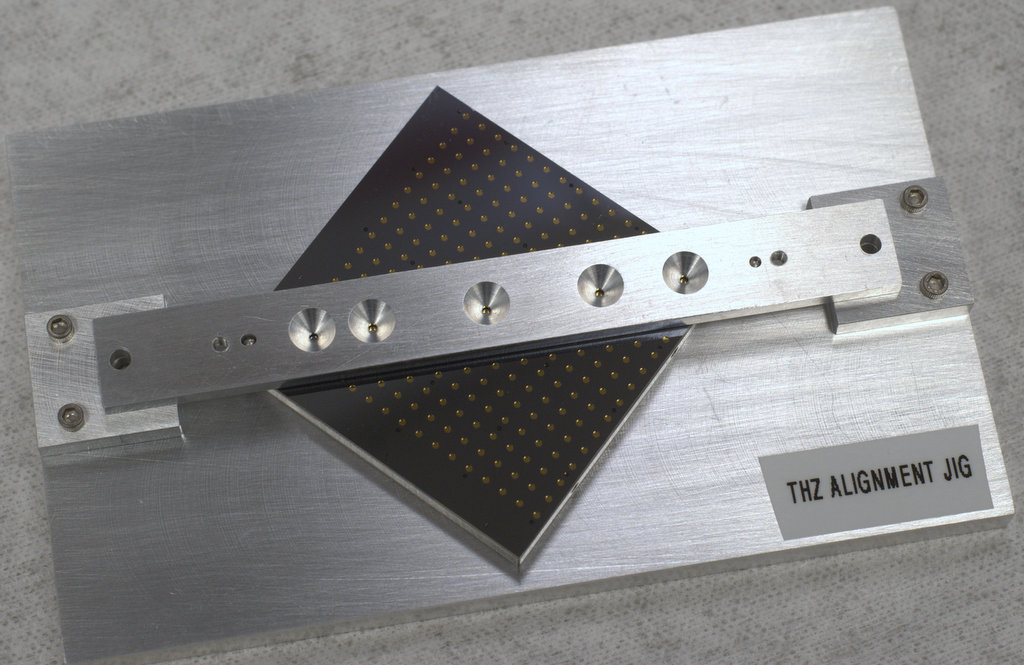
\includegraphics{drawings/ch5-alignment-jig.pdf}
\caption[Alignment jig]{
  Photograph of the alignment jig used to align the \Imager's sub-array to the Invar plate.
  The Invar plate and the metal bar are aligned to each other with dowel pins.
  The metal bar has conical cut-outs placed so that when detectors are aligned with them, the wafer is aligned properly to the Invar.
  In order to make it easy to move the detector wafer stack to the proper location, the entire assembly is warmed to \SI{30}{\celsius}; at this temperature the thermal grease thins.
}
\label{fig:ch5-alignment-jig}
\end{figure*}

Four 100-wire woven Phosphor Bronze wire harnesses run from \SI{300}{\K} to the focal plane, heat sunk along the way at the \SI{80}{\K} and \SI{6}{\K} stages.
These wires carry the readout signals to and from the \MCE.
Once they reach the focal plane a circuit board routes the wires to each sub-array.
One 100-wire harness carried the row-address wires and the circuit board routes the wires to all multiplexing chips in series (32 chips for the full array).
The other four 100-wire harnesses each carry \SQUID\ bias and feedback wires for a single sub-array.

To aid in routing of the wires, each sub-array has two ``wiring chips'' associated with it, visible in \figref{fig:ch5-focal-plane-platter}, and shown in schematic form in \figref{fig:ch5-wiring-chip-schematic}.
These chips aid in routing row-address and detector bias wires.
On top of each wiring chip are four multiplexing chips as well as four ``interface'' chips which contain Nyquist inductors and shunt resistors for the detectors.

\begin{figure*}
\centering
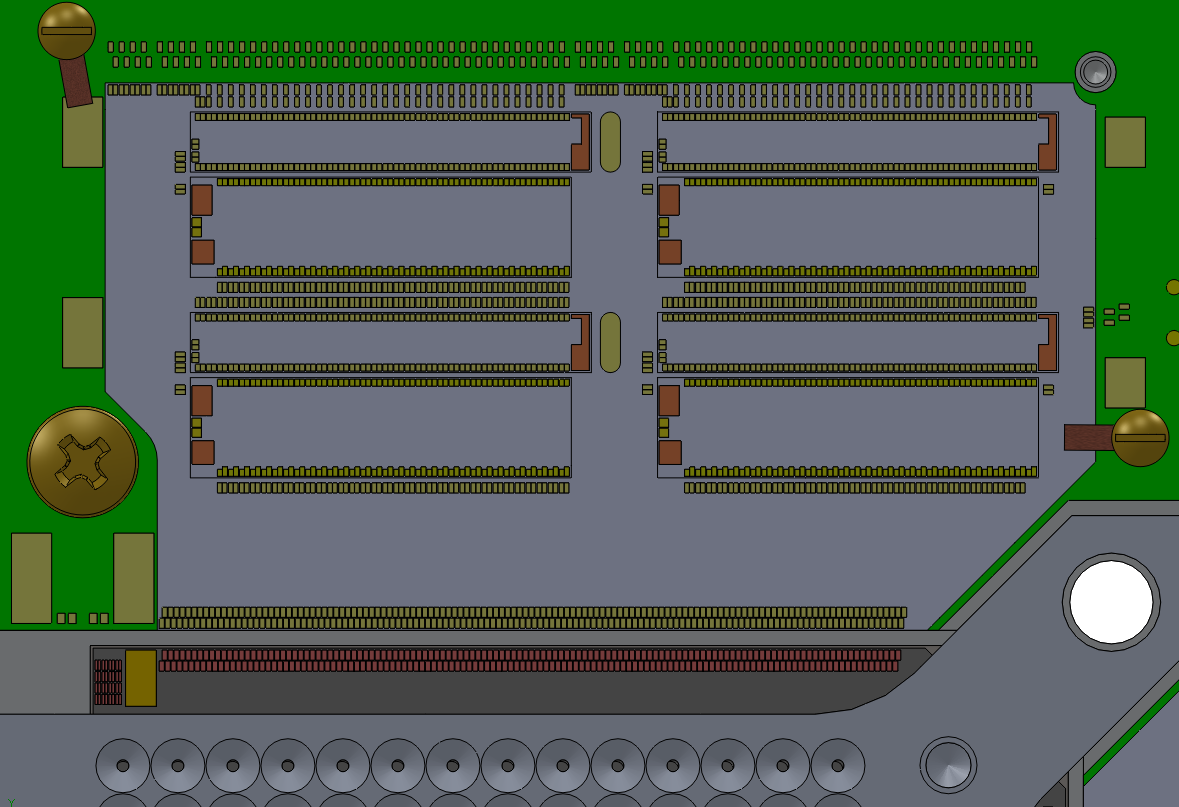
\includegraphics{drawings/ch5-wiring-chip-schematic.pdf}
\caption[Wiring chip schematic]{
  Schematic showing close-up view of the wiring chips with multiplexing and interface chips on top.
}
\label{fig:ch5-wiring-chip-schematic}
\end{figure*}

\begin{figure*}
\centering
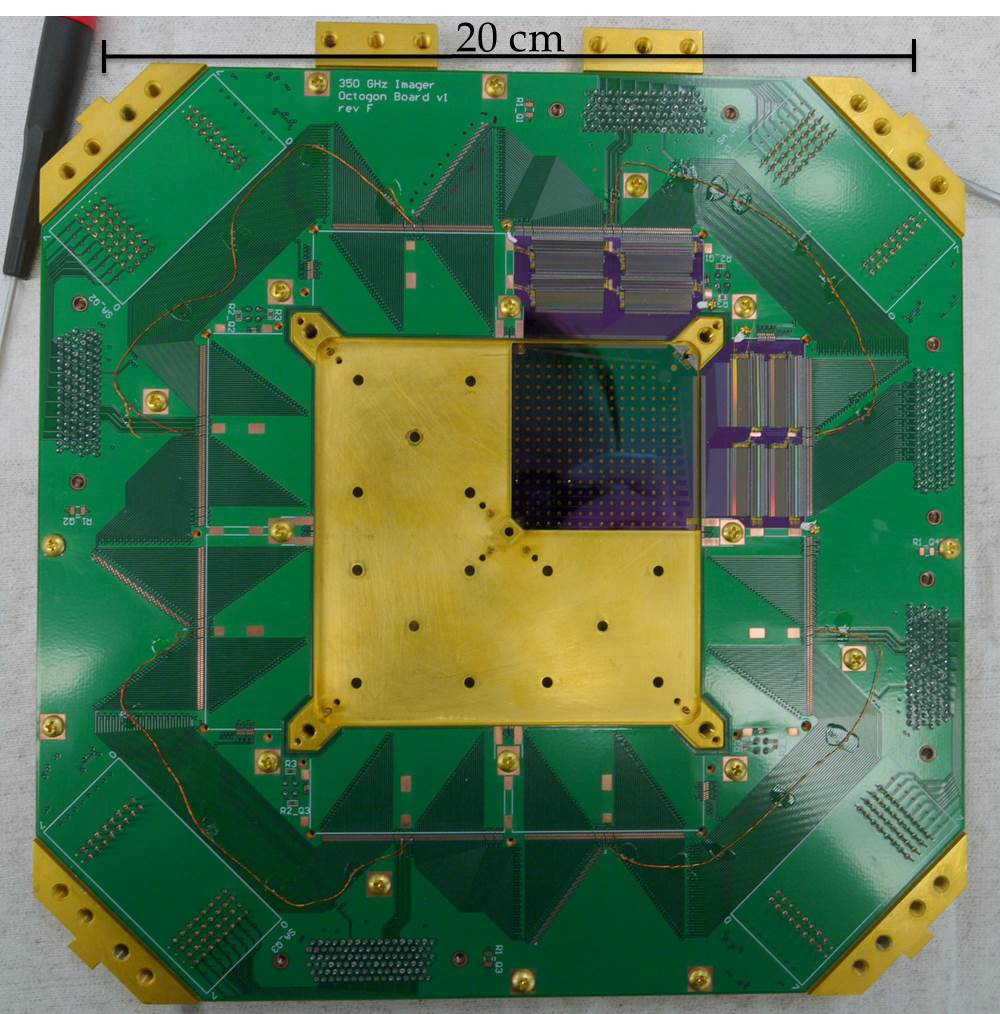
\includegraphics{drawings/ch5-focal-plane-platter.pdf}
\caption[Focal plane during assembly]{
  Photograph of the focal plane platter while being assembled.
  The platter was machined out of Al 6061 and then Au-plated.
  The green circuit board routes the 500 PhBr wires running from room temperature to the multiplexing and interface chips.
  The wiring chips (with multiplexing and interface chips on top) are labeled \textbf{A}, while the 251-detector sub-array is labeled \textbf{B}.
}
\label{fig:ch5-focal-plane-platter}
\end{figure*}

\section{System Field of View} \label{sec:ch5-fov}

We have now have enough information to calculate the total field of view of the \Imager.
As discussed in \sectionref{sec:ch7-focus-distance}, although the system is configured to focus at \SI{16}{\m}, the actual focal distance is \SI{17}{\m}, so I used values for that distance from \tableref{tab:ch4-zemax-parms}.
A \SI{1}{\mm} movement of the actuator produces a rotation of the secondary mirror of \ang{0.276}; a \ang{1.0} rotation of the secondary mirror displaces the beam of an on-axis detector by \SI{19.33}{\cm} at the far-field focal plane.

To convert actuator displacements into locations in the far-field, three additional factors should be considered.
First, the Cassegrain optical system inverts images that it views, so that a beam from a detector in the lower left of the focal plane (as viewed from behind the detector focal plane) is pointed to the upper right on the far-field image (again as viewed from the system).
Second, tilting the mirror displaces the beams in the same direction as the mirror is tilted; this is easily seen by thinking of the system in transmission, and imagining the way a ray of light is reflected off of a rotated mirror.
Third, the actuators are oriented so that their rotation axes are rotated from horizontal/vertical by \ang{45}.
This all means that --- as viewed from the cryostat --- positive displacements of the \DISP1 actuator shift beams up and to the right, while positive displacements of the \DISP2 actuator shift beams up and to the left.
If we consider an $x$-$y$ coordinate system in the far-field, this means that the $x$ and $y$ displacement of the beams due to mirror movements are calculated as
\begin{equation} \label{eqn:ch5-bose-to-x}
\Delta x = \frac{\sqrt{2}}{2} \left( d_{\text{DISP1}} - d_{\text{DISP2}} \right) \times
    \frac{\ang{0.276}} {\SI{1}{\mm}} \times
    \frac{\SI{19.33}{\cm}} {\ang{1}}
\end{equation}
\begin{equation} \label{eqn:ch5-bose-to-y}
\Delta y = \frac{\sqrt{2}}{2} \left( d_{\text{DISP1}} + d_{\text{DISP2}} \right) \times
    \frac{\ang{0.276}} {\SI{1}{\mm}} \times
    \frac{\SI{19.33}{\cm}} {\ang{1}}
\end{equation}
Here $d_{\text{DISP1}}$ and $d_{\text{DISP2}}$ are the displacements of the two actuators in \si{\mm}.

The maximum displacement of the \BOSE\ actuators is \SI{3.5}{\mm}.
Assuming a circular scan, the maximum far-field displacement of the on-axis point will be $\SI{3.5}{\mm} \times \SI[per-mode=symbol]{0.276}{\degree\per\mm} \times \SI[per-mode=symbol]{19.33}{\cm\per\degree} = \SI{18.7}{\cm}$.
When fully populated with 1004 detectors, the four sub-arrays cover an area $\SI{86}{\mm} \times \SI{86}{\mm}$, so the far-field radius of the circle covered by the detectors will be $\sqrt{2} \times (\SI{86}{\mm}/2) \times \SI{6.638}{\mm\per\mm} + \SI{18.7}{\cm} = \SI{55.8}{\cm}$, for a total area covered of \SI{.98}{\m^2}.
With a single 251-detector sub-array populated, the field of view will drop to \SI{0.42}{\m^2}.
If the scan is elliptical the areal field of view will be smaller still, though the elliptical shape may be more useful for some imaging scenarios.

\section{Predicted Noise} \label{sec:ch5-predicted-noise}

Using the targeted value of $G$ we can predict the total noise on the detectors as well as the expected \NETD\ in video images.
As discussed in \sectionref{sec:ch3-tes-noise}, intrinsic detector noise should be dominated by thermal fluctuation noise, given by
\begin{equation}
  S^2_{TFN} = 4 k_B T_0^2 G F(T_0, T_b).
\end{equation}
Using $G = \SI{3.8}{\nW\per\K}$, $T_0 = \SI{1.2}{\K}$, and $F = 0.83$ leads to $S_{TFN} = \Pnoisef{0.5}$.
This is \SI{60}{\percent} of \sectionref{sec:ch4-opt-eff}'s predicted photon noise of \Pnoisef{0.85}.
Summing the two noise sources in quadrature gives for the total noise (referred to power absorbed in the detector) $S_{tot} = \Pnoisef{1.0}$.

To estimate the \NETD\ achieved by the \Imager we use \eqnref{eqn:ch1-netd-defn}:
\begin{align}
  NETD = \frac{NEP}{\eta_{tot} M k_B \Delta \nu} \frac{1}{s} \sqrt{\frac{A\,FPS}{2 N}} .
\end{align}
With a fully-populated system of 1004 detectors sensitive to $M=2$ polarization modes, 20 frames per second, $A = \SI{1}{\m^2}$ from \sectionref{sec:ch5-fov}, and $ s = \SI{1}{\cm}$ resolution this leads to \NETD\ = \SI{38}{\mK}.
With a single sub-array populated \NETD\ would increase to \SI{50}{\mK}, with the smaller number of detectors increasing \NETD\ but the smaller field of view improving it. 

\section{Acknowledgments}

Hsiao-Mei (Sherry) Cho fabricated the detectors and wiring chips, as well as providing much useful advice during the design and layout of both.
The interface chips were designed --- and spares kindly donated --- by the \ABS\ team.
Jeff Van Lanen fabricated the backshort wafers and the Quantum Sensors Project \SQUID\ fabrication team made the multiplexing chips.
Colin Fitzgerald performed all wire bonding.
Lisa Ferreira did the soldering of the 100-pin MDM connectors to the circuit board, as well as a variety of other detail-oriented soldering tasks.
The idea to connect the focal plane the \SI{6}{\K} Cold Plate using the Ti-4Al-4V spiders was William Duncan's.
Ilya Smirnov carried out a series of simulations to investigate advantages of square vs hexagonal detector grids, as well as required detector time constants to avoid blurring.
Although these simulations are not discussed in this dissertation, they supported the conclusions of \sectionref{sec:det-parm-choice}.
